\documentclass[12pt]{article}

\usepackage{hyperref}
\usepackage{physics}
\usepackage{listings}
\usepackage{graphicx}
\usepackage{upgreek}
\usepackage{tgtermes}

\setcounter{tocdepth}{5}
\setcounter{secnumdepth}{4}

\title{Manual on the Code of the Book Entitled ``Acoustic Waves Generated by Parametric Array Loudspeakers''}
\author{Jiaxin Zhong}
\date{\today}

\begin{document}

\maketitle

\tableofcontents


\section{Introduction}
This document introduces the usage of the code package, which is a supplementary material for the book ``Acoustic Waves Generated by Parametric Array Loudspeakers''.
All demos and functions were tested by MATLAB R2022b installed on a personal computer with an AMD Ryzen Threadripper 3960X central processing unit (CPU) with 256 GB of random access memory (RAM).

\subsection{Installation}

Steps:
\begin{enumerate}
    \item Download all codes from \href{https://github.com/JiaxinZhong/AWPAL/}{GitHub: JiaxinZhong/AWPAL}
    \item Run the script AWPAL.m at first to add subfolders to the path.
\end{enumerate}





\section{Demo Scripts and Core Functions}

\subsection{Direct Integration Method (DIM)}

\subsubsection{Ultrasound Field}
\paragraph{General Solution}

\subparagraph{Function: \lstinline!DIM3D.m!}
The calculation utilizes the Rayleigh integral reading that \cite[Eq. (2.39)]{Zhong2024AcousticWavesGenerated}
\begin{equation}
    p_i(\vb{r})
    =
    \frac{\rho_0\omega_i}{2\uppi \mathrm{i} }
    \iint_{-\infty}^\infty
    v_{i,z}(\vb{r}_\mathrm{s})
    \frac{\mathrm{e}^{\mathrm{i} k_i \abs{\vb{r}-\vb{r}_\mathrm{s}}}}{\abs{\vb{r}-\vb{r}_\mathrm{s}}}
    \dd^2 \vb{r}_\mathrm{s}
    .
    \label{eq:Rayleigh_int:3ije23oi}
\end{equation}


\subsubsection{Audio Sound Field}

\paragraph{General Solution}

\subsubsection{Function: \lstinline!PalDIM3D.m!}
\begin{equation}
    p_\mathrm{a}(\vb{r})
    =
    -\frac{\beta\omega_\mathrm{a}^2}{4\uppi\rho_0c_0^4}
    \iiint_{-\infty}^\infty
    \frac{
        p_1^*(\vb{r}_\mathrm{v})
        p_2(\vb{r}_\mathrm{v})
    }{\abs{\vb{r}-\vb{r}_\mathrm{v}}}
    \mathrm{e}^{\mathrm{i} k_\mathrm{a} \abs{\vb{r}-\vb{r}_\mathrm{v}}}
    \dd^3 \vb{r}_\mathrm{v}
    .
    \label{eq:dim_3d_audio}
\end{equation}

\paragraph{On-Axis}

\subparagraph{Demo: \lstinline!PalDIM3D_CircSrc_Axis_Demo.m!}
Figure~\ref{fig:dim:uniform:32oj4} is generated by this demo file.
The data is stored in file \lstinline!PalDIM3D_CircSrc_Axis_Demo_Uniform.mat!.
\begin{figure}[!htb]
    \centering
    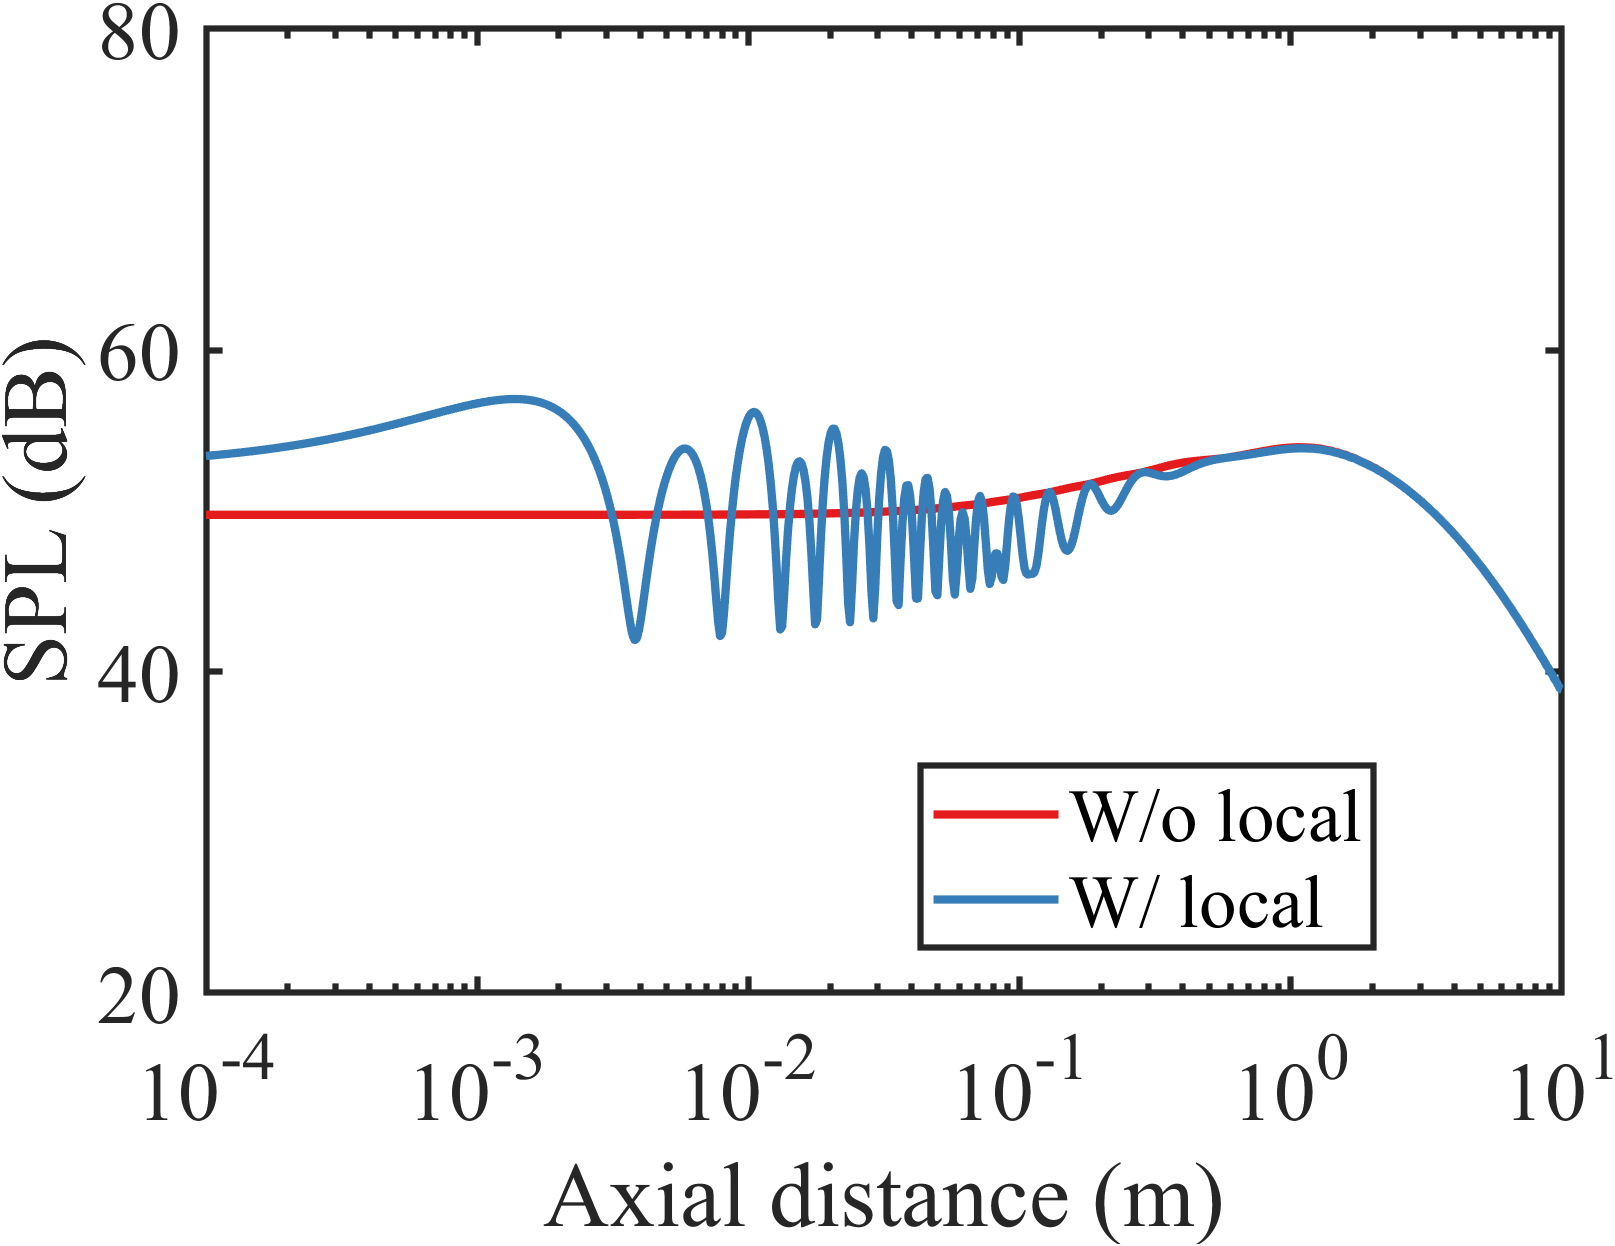
\includegraphics[width = 0.6\textwidth]{../code/DIM/fig/PalDIM3D_CircSrc_Axis_Demo_Uniform.png}
    \caption{On-axial SPL (dB) as a function of the axial distance ($z$, m) \cite[Fig.~2(d)]{Zhong2022LowFrequencyAudio}.
        The PAL has a circular uniform profile with a radius of $a=0.1\,\mathrm{m}$.
    }
    \label{fig:dim:uniform:32oj4}
\end{figure}

Figure~\ref{fig:dim:focus:32oj4} is generated by this demo file.
The data is stored in file \lstinline!PalDIM3D_CircSrc_Axis_Demo_Focus.mat!.
\begin{figure}[!htb]
    \centering
    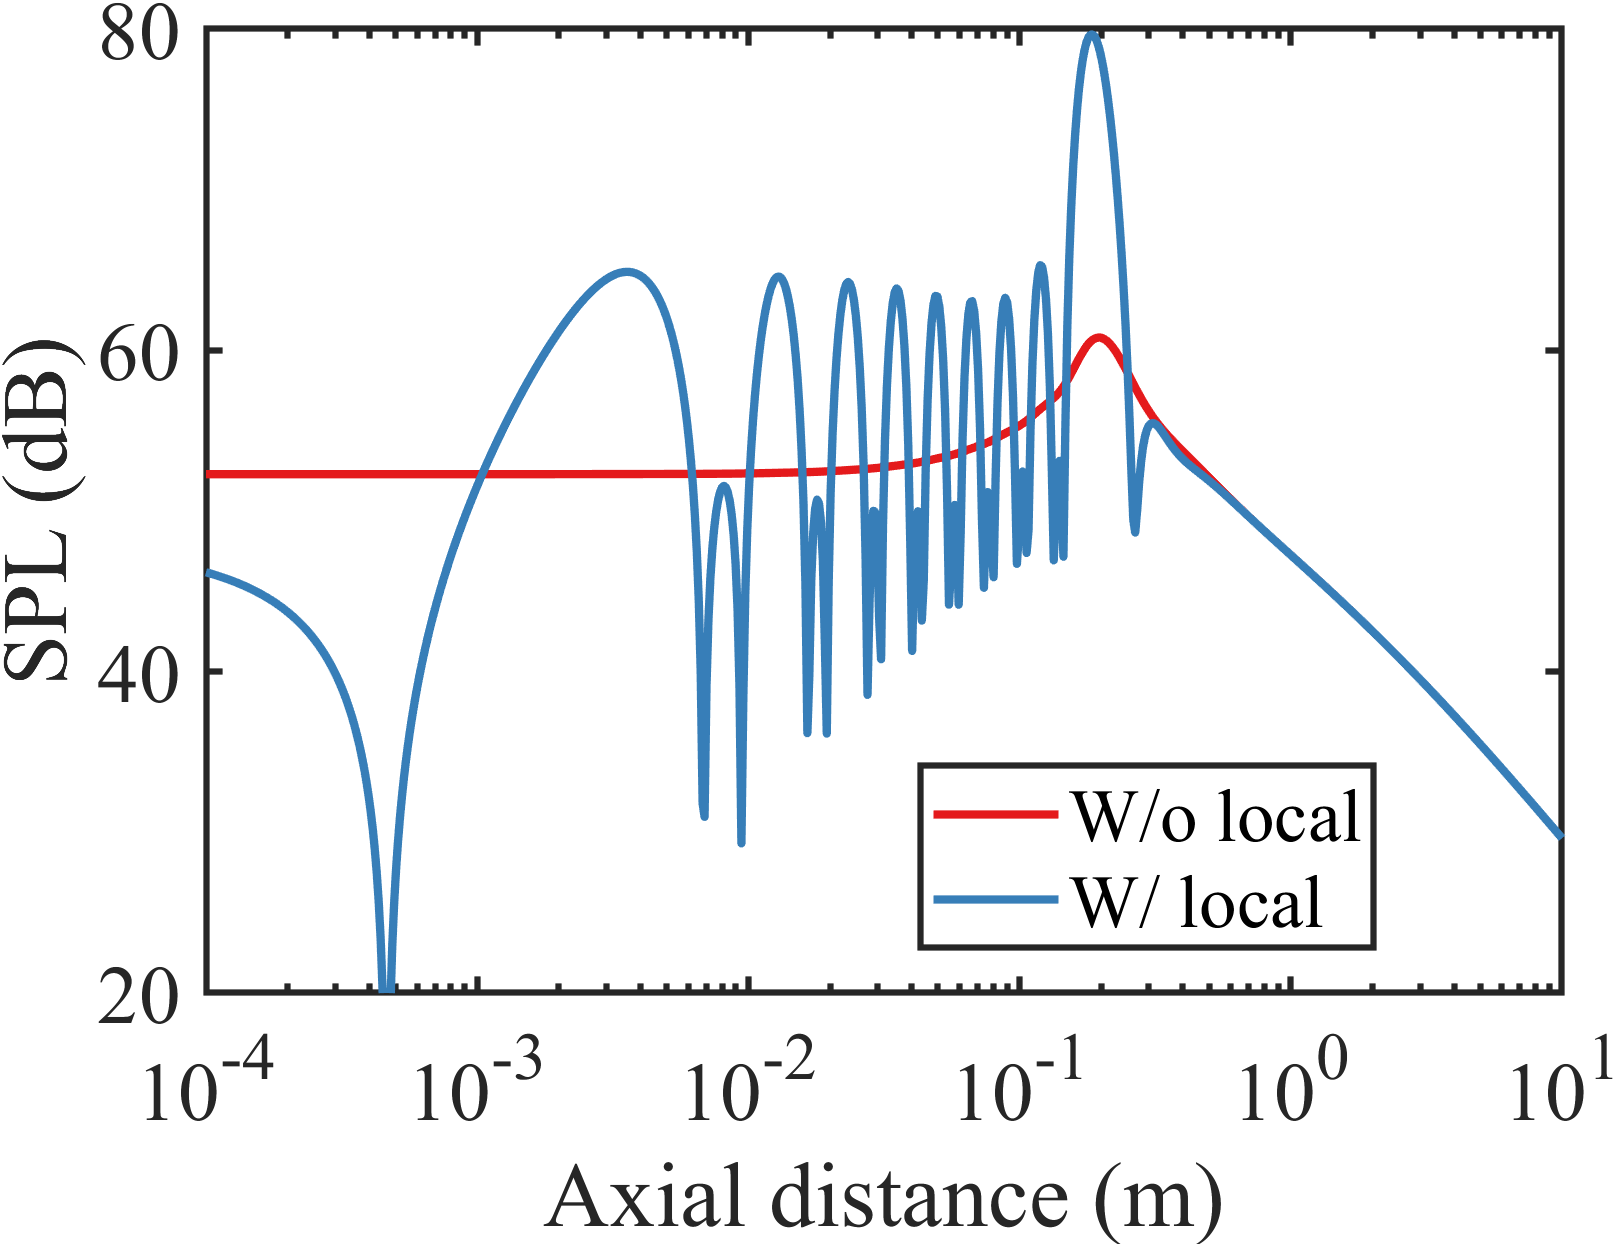
\includegraphics[width = 0.6\textwidth]{../code/DIM/fig/PalDIM3D_CircSrc_Axis_Demo_Focus.png}
    \caption{On-axial SPL (dB) as a function of the axial distance ($z$, m) \cite[Fig.~2(e)]{Zhong2022LowFrequencyAudio}.
        The PAL has a focusing profile with a focal distance of $r_\mathrm{f} = 0.2\,{m}$.
        The radius of the PAL is $a=0.1\,\mathrm{m}$.
    }
    \label{fig:dim:focus:32oj4}
\end{figure}

\subparagraph{Function: \lstinline!PalDIM3D_CircSrc_Axis.m!}
Calculate the audio sound field on the axis $\rho=0$ using the DIM.
The source profile is assumed to be axisymmetric in the azimuthal direction, i.e., $v_{i,z}(\vb{r}_\mathrm{s})$ is independent of $\varphi_\mathrm{s}$.
The formula used in this function is
\begin{equation}
    p_\mathrm{a}(\rho = 0, \varphi,z)
    =
    -\frac{\beta\omega_\mathrm{a}^2}{2\rho_0c_0^4}
    \int_{-\infty}^\infty \int_0^\infty
    \frac{p_1^*(\vb{r}_\mathrm{v})p_2(\vb{r}_\mathrm{v})}{\sqrt{\rho_\mathrm{v}^2 + (z-z_\mathrm{v})^2}} \mathrm{e}^{\mathrm{i}k_\mathrm{a} \sqrt{\rho_\mathrm{v}^2 + (z-z_\mathrm{v})^2}}
    \rho_\mathrm{v}\dd \rho_\mathrm{v}\dd z_\mathrm{v}
\end{equation}

\subsection{Spherical Wave Expansion (SWE)}

\subsubsection{Function: \lstinline!SWE3D_RadialInt.m!}
Calculate
\begin{equation}
    \int_{r_1}^{r_2}
    \mathrm{j}_n(kr_<)
    \mathrm{h}_n(kr_>)
    r_\mathrm{s}\dd r_\mathrm{s}
\end{equation}
where $r_<=\min(r,r_\mathrm{s})$ and $r_> = \max(r,r_\mathrm{s})$.



\section{Summary of Equations}

\subsection{Source Profile}

The focusing profile reads
\begin{equation}
    v_{i,z}(\vb{r}_\mathrm{s})
    =
    v_0 \exp\qty(-\mathrm{i} \real (k_i) \abs{\vb{r}_\mathrm{f} - \vb{r}_\mathrm{s}}).
\end{equation}
where $\vb{r}_\mathrm{f}$ denotes the location of the focal point.


\section{Known Issues}

\addcontentsline{toc}{section}{References}
\bibliographystyle{unsrt}
\bibliography{bibtex}


\end{document}